
%%% a book template designed for pdfLaTeX based upon video https://youtu.be/TyTx-BuLFh0
%%% created by Dan Liddell in July 2021.
%%%%%%%%%%%%%%%%%%%%%%%%%%%%%%%%%%%%%%%%%%%%%%%%%%%%%%%%%%%%%%%%%%%%%%%%
\documentclass[11pt,letterpaper]{book}
%%%%%%%%%%%%%%%%%%%%%%%%%%%%%%%%%%%%%%%%%%%%%%%%%%%%%%%%%%%%%%%%%%%%%%%%
%%% important packages
% improved tables
\usepackage{booktabs}
% improved caption handling
\usepackage[font=sf]{caption}
% font specification. use the original Computer Modern fonts.
\usepackage[T1]{fontenc}
% set margins
\usepackage[top=1.5in,bottom=1.25in,headheight=14pt]{geometry} % headheight is to override fancyhdr warning
% graphics handling
\usepackage{graphicx}
\graphicspath{{./graphics/}} % the graphics directory, so you only have to specify file basenames in figure references.
% index creation
\usepackage{makeidx}
\makeindex
% bibliography citations geared toward natural science publications
\usepackage[comma]{natbib}
% add index and bibliography to toc
% there appears to be a bug in the interaction of hyperref with tocbibind: the toc link to the index doesn't go to the proper page.
\usepackage{tocbibind}
% toc, lof, and lot support
\usepackage[titles]{tocloft}
% use sans-serif font for the frontmatter tables
\renewcommand{\cftchapfont}{\sffamily}
\renewcommand{\cftsecfont}{\sffamily}
\renewcommand{\cftchappagefont}{\sffamily}
\renewcommand{\cftsecpagefont}{\sffamily}
\renewcommand{\cftsubsecfont}{\sffamily}
\renewcommand{\cftsubsecpagefont}{\sffamily}
\renewcommand{\cftfigfont}{\sffamily}
\renewcommand{\cftfigpagefont}{\sffamily}
\renewcommand{\cfttabfont}{\sffamily}
\renewcommand{\cfttabpagefont}{\sffamily}
% extended color support
\usepackage[table,svgnames]{xcolor}

%%% include these if writing mathematics
% \usepackage{amsmath,amssymb,amsfonts}
% \usepackage{mathpmx}

%%%%%%%%%%%%% some advice about setting headers
% https://tex.stackexchange.com/questions/89914/chapter-name-in-the-header-with-chapter
% https://alvinalexander.com/blog/post/latex/get-chapter-name-section-name-inheader-of-page-in-latex-document/
%%%%%%%%%%%%%
% make sans-serif section headers
\usepackage{titlesec}
\titleformat{\chapter}{\sffamily\huge\bfseries}{}{0pt}{}
\titleformat{\section}{\sffamily\LARGE\mdseries}{}{0pt}{}
\titleformat{\subsection}{\sffamily\large\mdseries}{}{0pt}{}
% page header and footer management
\usepackage{fancyhdr}
\fancyhf{}
\renewcommand{\chaptermark}[1]{\markboth{#1}{}}
\renewcommand{\sectionmark}[1]{\markright{#1}}
\fancyhead[LE]{\sffamily\itshape\nouppercase{\rightmark}}
\fancyhead[RO]{\sffamily\bfseries\upshape\nouppercase{\leftmark}}
\fancyheadoffset[RE,LO]{-0.21\textwidth}
\pagestyle{fancy}
% make auto-generated blank pages empty
\usepackage{emptypage}
% or make them plain
% \makeatletter
% \def\cleardoublepage{\clearpage\if@twoside \ifodd\c@page\else
%	\hbox{}\thispagestyle{plain}\newpage\if@twocolumn\hbox{}\newpage\fi\fi\fi}
% \makeatother
% or make them empty

%%%%%%%%%%%%%%%%%%%%%%%%%%%%%%%%%%%%%%%%%%%%%%%%%%%%%%%%%%%%%%%%%%%%%%%%
%%% miscellaneous packages
%%%%%%%%%%%%%%%%%%%%%%%%%%%%%%%%%%%%%%%%%%%%%%%%%%%%%%%%%%%%%%%%%%%%%%%%
%%% for drafts
% enter filler text
\usepackage{lipsum}
% enable double spacing
% \usepackage{setspace}
%%% enable hypertext
% usual advice is to load this package last, but glossaries must follow it
% in order for glossary links to work properly.
\usepackage[colorlinks]{hyperref}
\hypersetup{
	colorlinks=true, % set true if you want colored links
	linktoc=all,     % set to all if you want both sections and subsections linked
	linkcolor=blue,  % choose some color if you want links to stand out
	citecolor=blue,
	urlcolor=blue
}
%%% Include glossary entries
% include a glossary
\usepackage[toc]{glossaries}
\newglossaryentry{latex}{name={LaTeX}, description={A document preparation system based upon TeX created by Leslie Lamport}}
\newglossaryentry{tex}{name={TeX}, description={A document preparation system created by Donald Knuth}}
\makeglossaries

\begin{document}
	
% frontmatter: half title, frontispiece, title, colophon (copyright), dedication, toc, lof, lot, preface, acknowledgements
\frontmatter
%%% half-title

\thispagestyle{empty} % turn off headers and pagination
{%
	\Large \raggedright \textbf{\LaTeX\ Book Template}
}
\clearpage

%%% fronticepiece
\thispagestyle{empty}

\begin{center}
	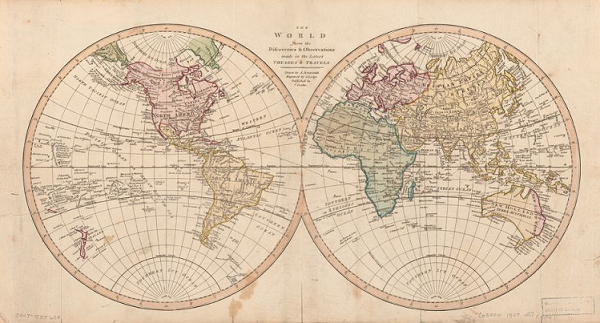
\includegraphics[width=0.7\linewidth]{world_map}
\end{center}

\vspace{-3ex}
\hspace{12em} {\footnotesize\textsf{Map courtesy of Library of Congress free-to-use images.}}
%%% title

\thispagestyle{empty}
{
\begin{center}
\Huge\bfseries\LaTeX\ Book Template\\[-1ex]
\rule{16.5pc}{0.5pt}\\[1in]
\LARGE\normalfont\textit{An Author}
\end{center}
}
%%% colophon

% remove headers and footers 
  \thispagestyle{plain}	

{ \clearpage 
  \raggedright
  \vspace*{5.5in}  
  \small\sffamily
  First edition 2021 by Dan Liddell\\[1em] 
  \begin{minipage}{0.85\linewidth}
  	This work is in the public domain and may be freely copied.\\
  	It is offered as-is with no guarantee or warranty of any sort.\\
  	If used as part of a publication, attribution to the author \\
  	is a reputable act.
  \end{minipage}
}
%%% dedication

% remove headers and footers 
\thispagestyle{plain}	

\clearpage
\null\vspace*{3in}
{\hfill \Large\itshape\ To all those who want to learn \LaTeX\ a bit better, including me.}
\vfill
% format toc depth to include section heads but no lower
\setcounter{tocdepth}{2}
\tableofcontents
\listoffigures
\listoftables
%%% preface

% remove headers and footers 
\thispagestyle{plain}	

\chapter{Preface}

This template was created in response to a number of requests found on various online forums for a \gls{latex} book template. Answers to such requests frequently offer unasked advice (sometimes almost sounding like admonishments for posting such queries) instead of providing  what was requested: a book template such as this. That being said, it is evident there are myriad considerations when putting together a book, let alone doing so in \LaTeX. No template could hope to address even a small fraction of those considerations in the detail that ultimately may be needed. Nevertheless, having a place to start can be beneficial to the novice. Who knows? An experienced \LaTeX\ author might even learn something by reviewing this material. But as it stands, this template is merely a starting point that may lend itself to an interesting foray into more extensive authoring. \vspace{3\parsep}

I gratefully acknowledge the work of the following people for making even this modest project possible: \index{Knuth, Donald} Donald Knuth and \index{Lamport, Leslie} Leslie Lamport for creating the foundation upon which the whole structure stands; Helmut Kopka and Patrick W. Daly for writing {\itshape Guide to \LaTeX}, from which I learned so much; Chandra Has for his excellent \LaTeX\ video series on YouTube; and the innumerable unsung heroes at projects like CTAN, \gls{tex}-LaTeX Stack Exchange, LaTeX.org, and other such websites, along with the developers who produce so much great code supporting the best software system for producing truly beautiful documents.

\vspace{0.75in}\hspace{4in}\textit{Dan Liddell}

% suppress enumeration of chapters, appendices, and sections
\setcounter{secnumdepth}{-1}

% mainmatter: parts and chapters
\mainmatter
% move the page numbers to the corners of page footers
\fancyfoot{}
\fancyfoot[RO]{\hfill\thepage}
\fancyfoot[LE]{\thepage\hfill}
% do it for initial pages in chapters also
\fancypagestyle{plain}{
  \fancyhf{}
  \fancyfoot[OR,LE]{\thepage}
  \renewcommand{\headrulewidth}{0pt}
  \renewcommand{\footrulewidth}{0pt}
}
%%% First chapter

\chapter{First Chapter}

\lipsum[1-2]

\section{First Section}

\lipsum[3-6]

\subsection{First Subsection}

\lipsum[9-10]

\subsection{Second Subsection}

\lipsum[11-12]

\section{Second Section}

\lipsum[17-20]
%%% Second chapter

\chapter{Second Chapter}

\lipsum[21-22]

\section{First Section}

\lipsum[23]

\begin{table}[h!]
	\begin{center}
		\caption{Leading caption}
		\label{tab1}
		\begin{tabular}{l||c||r|} \hline
			leftward & centered              & rightward\\
			\cline{2-3}
			left     & center \vline\ center & right\\
			\cline{2-3}
			left     & center                & right\\
			\hline
		\end{tabular}\\[0.5ex]
	\end{center}
\end{table}

\section{Second Section}

\lipsum[25]

\begin{figure}[h!]
	\begin{minipage}{5.9in}
	    {\mdseries\footnotesize\textsf{\hspace{14em}Map courtesy of Library of Congress free-to-use images.}}
		\begin{center}
			{\vspace{-1.5ex}}
			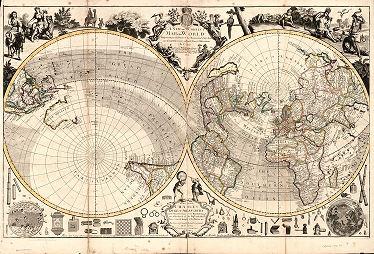
\includegraphics[width=0.62\linewidth]{world_map2}
		    \caption{Trailing caption}
		    \label{fig:map2} 
	    \end{center}
    \end{minipage}
\end{figure}



%%% Third chapter

\chapter{Third Chapter}

\lipsum[23-30]

\section{First Section}

\lipsum[33]

\begin{table}[!ht]
	\begin{center}
		\caption{Continent sizes}
		\index{continents}
		\label{tab2}
        \begin{tabular}{lr}
	       \rowcolor{Moccasin} \multicolumn{2}{c}{\bfseries Continental Areas {\small(sq. mi.)}}\\
	       \hline
           Asia    & 17,212,000\\
	       Africa  & 11,608,000\\
	       North America  & 9,365,000\\
	       South America  & 6,880,000\\
	       Antarctica     & 5,100,000\\
	       Europe         & 3,837,000\\
	       Australia      & 2,967,908\\
        \end{tabular}
	\end{center}
\end{table}

\section{Second Section}

\lipsum[34]

\begin{figure}[!ht]
	\begin{minipage}{5.9in}
		{\mdseries\footnotesize\textsf{\hspace{19.25em}Map courtesy of Library of Congress free-to-use images.}}
		\begin{center}
			{\vspace{-1.5ex}}
			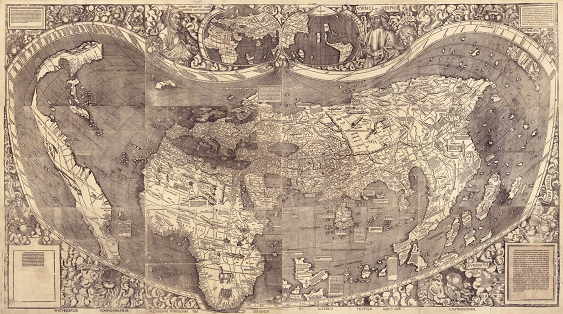
\includegraphics[width=0.85\linewidth]{world_map3}
			\caption{Cartograph}
			\label{fig:map3} 
		\end{center}
	\end{minipage}
\end{figure}
\appendix
%%% appendix

\chapter{Appendix}

\lipsum[42]

\section{Appx First Section}

\lipsum[43-54]

\section{Appx Second Section}

\lipsum[55]

% backmatter: appendices, bibliography, index, postface
\backmatter 
% change back to centered page numbers in roman numerals
\renewcommand{\thepage}{\roman{page}}
\fancypagestyle{plain}{
	\fancyhf{} % clear all header and footer fields
	\fancyfoot[C]{\thepage}
	\renewcommand{\headrulewidth}{0pt}
	\renewcommand{\footrulewidth}{0pt}
}
\printglossary
\bibliographystyle{plainnat}
% if not using tocbibind: \addcontentsline{toc}{chapter}{Bibliography}
\bibliography{backmatter/biblio}
{
% make the index in the current configuration start on an odd page.
% this can be better handled with ifoddpage package.
  \cleardoublepage
% use sans-serif face for index entries to match frontmatter auto-generated lists
% if not using tocbibind: \addcontentsline{toc}{chapter}{Index}
  \sffamily 
  \printindex
% print blank reverse page for current configuration of the index.
  \cleardoublepage
}
%%% postface

\thispagestyle{empty}
\small\sffamily
\begin{minipage}{5.5in}
This document was created using TeXstudio, compiled using PdfLaTeX and BibTeX, and typeset in Computer Modern. \vspace{3\parsep}

A generous amount of credit goes to these resources for providing the necessary information to produce this work: \citeauthor{Has,KnD}, and \citeauthor{Lam}.
\end{minipage}
	
%%% front cover, spline, backcover	
	
\end{document}
